\documentclass{article}


\usepackage{algorithm}
\usepackage{algpseudocode}

\usepackage{microtype}
\usepackage{lettrine}
\usepackage{hyperref}
\usepackage{threeparttable}
\usepackage{siunitx}
\usepackage{booktabs}
\usepackage[bitstream-charter]{mathdesign}
\usepackage{XCharter}
\usepackage[T1]{fontenc}
\usepackage{natbib}
\usepackage{mathtools}

\usepackage{tikz}
\usepackage{pgfplots}
\pgfplotsset{compat=newest}
\usepgfplotslibrary{groupplots}
\usetikzlibrary{external}
\usetikzlibrary{positioning, shapes, fit, 3d, perspective, shadings, intersections}

%%%%% NEW MATH DEFINITIONS %%%%%

\usepackage{amsmath,bm}

% Mark sections of captions for referring to divisions of figures
\newcommand{\figleft}{{\em (Left)}}
\newcommand{\figcenter}{{\em (Center)}}
\newcommand{\figright}{{\em (Right)}}
\newcommand{\figtop}{{\em (Top)}}
\newcommand{\figbottom}{{\em (Bottom)}}
\newcommand{\captiona}{{\em (a)}}
\newcommand{\captionb}{{\em (b)}}
\newcommand{\captionc}{{\em (c)}}
\newcommand{\captiond}{{\em (d)}}

% Highlight a newly defined term
\newcommand{\newterm}[1]{{\bf #1}}


% Figure reference, lower-case.
\def\figref#1{figure~\ref{#1}}
% Figure reference, capital. For start of sentence
\def\Figref#1{Figure~\ref{#1}}
\def\twofigref#1#2{figures \ref{#1} and \ref{#2}}
\def\quadfigref#1#2#3#4{figures \ref{#1}, \ref{#2}, \ref{#3} and \ref{#4}}
% Section reference, lower-case.
\def\secref#1{section~\ref{#1}}
% Section reference, capital.
\def\Secref#1{Section~\ref{#1}}
% Reference to two sections.
\def\twosecrefs#1#2{sections \ref{#1} and \ref{#2}}
% Reference to three sections.
\def\secrefs#1#2#3{sections \ref{#1}, \ref{#2} and \ref{#3}}
% Reference to an equation, lower-case.
\def\eqref#1{equation~\ref{#1}}
% Reference to an equation, upper case
\def\Eqref#1{Equation~\ref{#1}}
% A raw reference to an equation---avoid using if possible
\def\plaineqref#1{\ref{#1}}
% Reference to a chapter, lower-case.
\def\chapref#1{chapter~\ref{#1}}
% Reference to an equation, upper case.
\def\Chapref#1{Chapter~\ref{#1}}
% Reference to a range of chapters
\def\rangechapref#1#2{chapters\ref{#1}--\ref{#2}}
% Reference to an algorithm, lower-case.
\def\algref#1{algorithm~\ref{#1}}
% Reference to an algorithm, upper case.
\def\Algref#1{Algorithm~\ref{#1}}
\def\twoalgref#1#2{algorithms \ref{#1} and \ref{#2}}
\def\Twoalgref#1#2{Algorithms \ref{#1} and \ref{#2}}
% Reference to a part, lower case
\def\partref#1{part~\ref{#1}}
% Reference to a part, upper case
\def\Partref#1{Part~\ref{#1}}
\def\twopartref#1#2{parts \ref{#1} and \ref{#2}}

\def\ceil#1{\lceil #1 \rceil}
\def\floor#1{\lfloor #1 \rfloor}
\def\1{\bm{1}}
\newcommand{\train}{\mathcal{D}}
\newcommand{\valid}{\mathcal{D_{\mathrm{valid}}}}
\newcommand{\test}{\mathcal{D_{\mathrm{test}}}}

\def\eps{{\epsilon}}


% Random variables
\def\reta{{\textnormal{$\eta$}}}
\def\ra{{\textnormal{a}}}
\def\rb{{\textnormal{b}}}
\def\rc{{\textnormal{c}}}
\def\rd{{\textnormal{d}}}
\def\re{{\textnormal{e}}}
\def\rf{{\textnormal{f}}}
\def\rg{{\textnormal{g}}}
\def\rh{{\textnormal{h}}}
\def\ri{{\textnormal{i}}}
\def\rj{{\textnormal{j}}}
\def\rk{{\textnormal{k}}}
\def\rl{{\textnormal{l}}}
% rm is already a command, just don't name any random variables m
\def\rn{{\textnormal{n}}}
\def\ro{{\textnormal{o}}}
\def\rp{{\textnormal{p}}}
\def\rq{{\textnormal{q}}}
\def\rr{{\textnormal{r}}}
\def\rs{{\textnormal{s}}}
\def\rt{{\textnormal{t}}}
\def\ru{{\textnormal{u}}}
\def\rv{{\textnormal{v}}}
\def\rw{{\textnormal{w}}}
\def\rx{{\textnormal{x}}}
\def\ry{{\textnormal{y}}}
\def\rz{{\textnormal{z}}}

% Random vectors
\def\rvepsilon{{\mathbf{\epsilon}}}
\def\rvtheta{{\mathbf{\theta}}}
\def\rva{{\mathbf{a}}}
\def\rvb{{\mathbf{b}}}
\def\rvc{{\mathbf{c}}}
\def\rvd{{\mathbf{d}}}
\def\rve{{\mathbf{e}}}
\def\rvf{{\mathbf{f}}}
\def\rvg{{\mathbf{g}}}
\def\rvh{{\mathbf{h}}}
\def\rvu{{\mathbf{i}}}
\def\rvj{{\mathbf{j}}}
\def\rvk{{\mathbf{k}}}
\def\rvl{{\mathbf{l}}}
\def\rvm{{\mathbf{m}}}
\def\rvn{{\mathbf{n}}}
\def\rvo{{\mathbf{o}}}
\def\rvp{{\mathbf{p}}}
\def\rvq{{\mathbf{q}}}
\def\rvr{{\mathbf{r}}}
\def\rvs{{\mathbf{s}}}
\def\rvt{{\mathbf{t}}}
\def\rvu{{\mathbf{u}}}
\def\rvv{{\mathbf{v}}}
\def\rvw{{\mathbf{w}}}
\def\rvx{{\mathbf{x}}}
\def\rvy{{\mathbf{y}}}
\def\rvz{{\mathbf{z}}}

% Elements of random vectors
\def\erva{{\textnormal{a}}}
\def\ervb{{\textnormal{b}}}
\def\ervc{{\textnormal{c}}}
\def\ervd{{\textnormal{d}}}
\def\erve{{\textnormal{e}}}
\def\ervf{{\textnormal{f}}}
\def\ervg{{\textnormal{g}}}
\def\ervh{{\textnormal{h}}}
\def\ervi{{\textnormal{i}}}
\def\ervj{{\textnormal{j}}}
\def\ervk{{\textnormal{k}}}
\def\ervl{{\textnormal{l}}}
\def\ervm{{\textnormal{m}}}
\def\ervn{{\textnormal{n}}}
\def\ervo{{\textnormal{o}}}
\def\ervp{{\textnormal{p}}}
\def\ervq{{\textnormal{q}}}
\def\ervr{{\textnormal{r}}}
\def\ervs{{\textnormal{s}}}
\def\ervt{{\textnormal{t}}}
\def\ervu{{\textnormal{u}}}
\def\ervv{{\textnormal{v}}}
\def\ervw{{\textnormal{w}}}
\def\ervx{{\textnormal{x}}}
\def\ervy{{\textnormal{y}}}
\def\ervz{{\textnormal{z}}}

% Random matrices
\def\rmA{{\mathbf{A}}}
\def\rmB{{\mathbf{B}}}
\def\rmC{{\mathbf{C}}}
\def\rmD{{\mathbf{D}}}
\def\rmE{{\mathbf{E}}}
\def\rmF{{\mathbf{F}}}
\def\rmG{{\mathbf{G}}}
\def\rmH{{\mathbf{H}}}
\def\rmI{{\mathbf{I}}}
\def\rmJ{{\mathbf{J}}}
\def\rmK{{\mathbf{K}}}
\def\rmL{{\mathbf{L}}}
\def\rmM{{\mathbf{M}}}
\def\rmN{{\mathbf{N}}}
\def\rmO{{\mathbf{O}}}
\def\rmP{{\mathbf{P}}}
\def\rmQ{{\mathbf{Q}}}
\def\rmR{{\mathbf{R}}}
\def\rmS{{\mathbf{S}}}
\def\rmT{{\mathbf{T}}}
\def\rmU{{\mathbf{U}}}
\def\rmV{{\mathbf{V}}}
\def\rmW{{\mathbf{W}}}
\def\rmX{{\mathbf{X}}}
\def\rmY{{\mathbf{Y}}}
\def\rmZ{{\mathbf{Z}}}

% Elements of random matrices
\def\ermA{{\textnormal{A}}}
\def\ermB{{\textnormal{B}}}
\def\ermC{{\textnormal{C}}}
\def\ermD{{\textnormal{D}}}
\def\ermE{{\textnormal{E}}}
\def\ermF{{\textnormal{F}}}
\def\ermG{{\textnormal{G}}}
\def\ermH{{\textnormal{H}}}
\def\ermI{{\textnormal{I}}}
\def\ermJ{{\textnormal{J}}}
\def\ermK{{\textnormal{K}}}
\def\ermL{{\textnormal{L}}}
\def\ermM{{\textnormal{M}}}
\def\ermN{{\textnormal{N}}}
\def\ermO{{\textnormal{O}}}
\def\ermP{{\textnormal{P}}}
\def\ermQ{{\textnormal{Q}}}
\def\ermR{{\textnormal{R}}}
\def\ermS{{\textnormal{S}}}
\def\ermT{{\textnormal{T}}}
\def\ermU{{\textnormal{U}}}
\def\ermV{{\textnormal{V}}}
\def\ermW{{\textnormal{W}}}
\def\ermX{{\textnormal{X}}}
\def\ermY{{\textnormal{Y}}}
\def\ermZ{{\textnormal{Z}}}

% Vectors
\def\vzero{{\bm{0}}}
\def\vone{{\bm{1}}}
\def\vmu{{\bm{\mu}}}
\def\vtheta{{\bm{\theta}}}
\def\va{{\bm{a}}}
\def\vb{{\bm{b}}}
\def\vc{{\bm{c}}}
\def\vd{{\bm{d}}}
\def\ve{{\bm{e}}}
\def\vf{{\bm{f}}}
\def\vg{{\bm{g}}}
\def\vh{{\bm{h}}}
\def\vi{{\bm{i}}}
\def\vj{{\bm{j}}}
\def\vk{{\bm{k}}}
\def\vl{{\bm{l}}}
\def\vell{{\bm{\ell}}}
\def\vm{{\bm{m}}}
\def\vn{{\bm{n}}}
\def\vo{{\bm{o}}}
\def\vp{{\bm{p}}}
\def\vq{{\bm{q}}}
\def\vr{{\bm{r}}}
\def\vs{{\bm{s}}}
\def\vt{{\bm{t}}}
\def\vu{{\bm{u}}}
\def\vv{{\bm{v}}}
\def\vw{{\bm{w}}}
\def\vx{{\bm{x}}}
\def\vy{{\bm{y}}}
\def\vz{{\bm{z}}}

% Elements of vectors
\def\evalpha{{\alpha}}
\def\evbeta{{\beta}}
\def\evepsilon{{\epsilon}}
\def\evlambda{{\lambda}}
\def\evomega{{\omega}}
\def\evmu{{\mu}}
\def\evpsi{{\psi}}
\def\evsigma{{\sigma}}
\def\evtheta{{\theta}}
\def\eva{{a}}
\def\evb{{b}}
\def\evc{{c}}
\def\evd{{d}}
\def\eve{{e}}
\def\evf{{f}}
\def\evg{{g}}
\def\evh{{h}}
\def\evi{{i}}
\def\evj{{j}}
\def\evk{{k}}
\def\evl{{l}}
\def\evm{{m}}
\def\evn{{n}}
\def\evo{{o}}
\def\evp{{p}}
\def\evq{{q}}
\def\evr{{r}}
\def\evs{{s}}
\def\evt{{t}}
\def\evu{{u}}
\def\evv{{v}}
\def\evw{{w}}
\def\evx{{x}}
\def\evy{{y}}
\def\evz{{z}}

% Matrix
\def\mA{{\bm{A}}}
\def\mB{{\bm{B}}}
\def\mC{{\bm{C}}}
\def\mD{{\bm{D}}}
\def\mE{{\bm{E}}}
\def\mF{{\bm{F}}}
\def\mG{{\bm{G}}}
\def\mH{{\bm{H}}}
\def\mI{{\bm{I}}}
\def\mJ{{\bm{J}}}
\def\mK{{\bm{K}}}
\def\mL{{\bm{L}}}
\def\mM{{\bm{M}}}
\def\mN{{\bm{N}}}
\def\mO{{\bm{O}}}
\def\mP{{\bm{P}}}
\def\mQ{{\bm{Q}}}
\def\mR{{\bm{R}}}
\def\mS{{\bm{S}}}
\def\mT{{\bm{T}}}
\def\mU{{\bm{U}}}
\def\mV{{\bm{V}}}
\def\mW{{\bm{W}}}
\def\mX{{\bm{X}}}
\def\mY{{\bm{Y}}}
\def\mZ{{\bm{Z}}}
\def\mBeta{{\bm{\beta}}}
\def\mPhi{{\bm{\Phi}}}
\def\mLambda{{\bm{\Lambda}}}
\def\mSigma{{\bm{\Sigma}}}

% Tensor
\DeclareMathAlphabet{\mathsfit}{\encodingdefault}{\sfdefault}{m}{sl}
\SetMathAlphabet{\mathsfit}{bold}{\encodingdefault}{\sfdefault}{bx}{n}
\newcommand{\tens}[1]{\bm{\mathsfit{#1}}}
\def\tA{{\tens{A}}}
\def\tB{{\tens{B}}}
\def\tC{{\tens{C}}}
\def\tD{{\tens{D}}}
\def\tE{{\tens{E}}}
\def\tF{{\tens{F}}}
\def\tG{{\tens{G}}}
\def\tH{{\tens{H}}}
\def\tI{{\tens{I}}}
\def\tJ{{\tens{J}}}
\def\tK{{\tens{K}}}
\def\tL{{\tens{L}}}
\def\tM{{\tens{M}}}
\def\tN{{\tens{N}}}
\def\tO{{\tens{O}}}
\def\tP{{\tens{P}}}
\def\tQ{{\tens{Q}}}
\def\tR{{\tens{R}}}
\def\tS{{\tens{S}}}
\def\tT{{\tens{T}}}
\def\tU{{\tens{U}}}
\def\tV{{\tens{V}}}
\def\tW{{\tens{W}}}
\def\tX{{\tens{X}}}
\def\tY{{\tens{Y}}}
\def\tZ{{\tens{Z}}}


% Graph
\def\gA{{\mathcal{A}}}
\def\gB{{\mathcal{B}}}
\def\gC{{\mathcal{C}}}
\def\gD{{\mathcal{D}}}
\def\gE{{\mathcal{E}}}
\def\gF{{\mathcal{F}}}
\def\gG{{\mathcal{G}}}
\def\gH{{\mathcal{H}}}
\def\gI{{\mathcal{I}}}
\def\gJ{{\mathcal{J}}}
\def\gK{{\mathcal{K}}}
\def\gL{{\mathcal{L}}}
\def\gM{{\mathcal{M}}}
\def\gN{{\mathcal{N}}}
\def\gO{{\mathcal{O}}}
\def\gP{{\mathcal{P}}}
\def\gQ{{\mathcal{Q}}}
\def\gR{{\mathcal{R}}}
\def\gS{{\mathcal{S}}}
\def\gT{{\mathcal{T}}}
\def\gU{{\mathcal{U}}}
\def\gV{{\mathcal{V}}}
\def\gW{{\mathcal{W}}}
\def\gX{{\mathcal{X}}}
\def\gY{{\mathcal{Y}}}
\def\gZ{{\mathcal{Z}}}

% Sets
\def\sA{{\mathbb{A}}}
\def\sB{{\mathbb{B}}}
\def\sC{{\mathbb{C}}}
\def\sD{{\mathbb{D}}}
% Don't use a set called E, because this would be the same as our symbol
% for expectation.
\def\sF{{\mathbb{F}}}
\def\sG{{\mathbb{G}}}
\def\sH{{\mathbb{H}}}
\def\sI{{\mathbb{I}}}
\def\sJ{{\mathbb{J}}}
\def\sK{{\mathbb{K}}}
\def\sL{{\mathbb{L}}}
\def\sM{{\mathbb{M}}}
\def\sN{{\mathbb{N}}}
\def\sO{{\mathbb{O}}}
\def\sP{{\mathbb{P}}}
\def\sQ{{\mathbb{Q}}}
\def\sR{{\mathbb{R}}}
\def\sS{{\mathbb{S}}}
\def\sT{{\mathbb{T}}}
\def\sU{{\mathbb{U}}}
\def\sV{{\mathbb{V}}}
\def\sW{{\mathbb{W}}}
\def\sX{{\mathbb{X}}}
\def\sY{{\mathbb{Y}}}
\def\sZ{{\mathbb{Z}}}

% Entries of a matrix
\def\emLambda{{\Lambda}}
\def\emA{{A}}
\def\emB{{B}}
\def\emC{{C}}
\def\emD{{D}}
\def\emE{{E}}
\def\emF{{F}}
\def\emG{{G}}
\def\emH{{H}}
\def\emI{{I}}
\def\emJ{{J}}
\def\emK{{K}}
\def\emL{{L}}
\def\emM{{M}}
\def\emN{{N}}
\def\emO{{O}}
\def\emP{{P}}
\def\emQ{{Q}}
\def\emR{{R}}
\def\emS{{S}}
\def\emT{{T}}
\def\emU{{U}}
\def\emV{{V}}
\def\emW{{W}}
\def\emX{{X}}
\def\emY{{Y}}
\def\emZ{{Z}}
\def\emSigma{{\Sigma}}

% entries of a tensor
% Same font as tensor, without \bm wrapper
\newcommand{\etens}[1]{\mathsfit{#1}}
\def\etLambda{{\etens{\Lambda}}}
\def\etA{{\etens{A}}}
\def\etB{{\etens{B}}}
\def\etC{{\etens{C}}}
\def\etD{{\etens{D}}}
\def\etE{{\etens{E}}}
\def\etF{{\etens{F}}}
\def\etG{{\etens{G}}}
\def\etH{{\etens{H}}}
\def\etI{{\etens{I}}}
\def\etJ{{\etens{J}}}
\def\etK{{\etens{K}}}
\def\etL{{\etens{L}}}
\def\etM{{\etens{M}}}
\def\etN{{\etens{N}}}
\def\etO{{\etens{O}}}
\def\etP{{\etens{P}}}
\def\etQ{{\etens{Q}}}
\def\etR{{\etens{R}}}
\def\etS{{\etens{S}}}
\def\etT{{\etens{T}}}
\def\etU{{\etens{U}}}
\def\etV{{\etens{V}}}
\def\etW{{\etens{W}}}
\def\etX{{\etens{X}}}
\def\etY{{\etens{Y}}}
\def\etZ{{\etens{Z}}}

% The true underlying data generating distribution
\newcommand{\pdata}{p_{\rm{data}}}
% The empirical distribution defined by the training set
\newcommand{\ptrain}{\hat{p}_{\rm{data}}}
\newcommand{\Ptrain}{\hat{P}_{\rm{data}}}
% The model distribution
\newcommand{\pmodel}{p_{\rm{model}}}
\newcommand{\Pmodel}{P_{\rm{model}}}
\newcommand{\ptildemodel}{\tilde{p}_{\rm{model}}}
% Stochastic autoencoder distributions
\newcommand{\pencode}{p_{\rm{encoder}}}
\newcommand{\pdecode}{p_{\rm{decoder}}}
\newcommand{\precons}{p_{\rm{reconstruct}}}

\newcommand{\laplace}{\mathrm{Laplace}} % Laplace distribution

\newcommand{\E}{\mathbb{E}}
\newcommand{\Ls}{\mathcal{L}}
\newcommand{\R}{\mathbb{R}}
\newcommand{\emp}{\tilde{p}}
\newcommand{\lr}{\alpha}
\newcommand{\reg}{\lambda}
\newcommand{\rect}{\mathrm{rectifier}}
\newcommand{\softmax}{\mathrm{softmax}}
\newcommand{\sigmoid}{\sigma}
\newcommand{\softplus}{\zeta}
\newcommand{\KL}{D_{\mathrm{KL}}}
\newcommand{\Var}{\mathrm{Var}}
\newcommand{\standarderror}{\mathrm{SE}}
\newcommand{\Cov}{\mathrm{Cov}}
% Wolfram Mathworld says $L^2$ is for function spaces and $\ell^2$ is for vectors
% But then they seem to use $L^2$ for vectors throughout the site, and so does
% wikipedia.
\newcommand{\normlzero}{L^0}
\newcommand{\normlone}{L^1}
\newcommand{\normltwo}{L^2}
\newcommand{\normlp}{L^p}
\newcommand{\normmax}{L^\infty}

\newcommand{\parents}{Pa} % See usage in notation.tex. Chosen to match Daphne's book.

\DeclareMathOperator*{\argmax}{arg\,max}
\DeclareMathOperator*{\argmin}{arg\,min}

\DeclareMathOperator{\sign}{sign}
\DeclareMathOperator{\Tr}{Tr}
\let\ab\allowbreak

\newcommand\layernorm{\mathrm{layernorm}}
\newcommand\standardize{\mathrm{standardize}}
\newcommand\logits{\mathrm{logits}}
\newcommand\diag{\mathrm{diag}}
\newcommand\linalgspan{\mathrm{span}}

\author{Matthew Finlayson}
\title{Taking API-Protected Language Model Attacks One Layer Deeper}
\date{}

\begin{document}
\maketitle

\begin{abstract}
  To protect trade secrets, 
  language model (LM) providers often limit access to their models
  by exposing them only via a restrictive API.
  Recent work showed that under certain common configurations 
  these APIs leak non-public information 
  about their underlying LM architectures,
  such as the model's embedding size.
  The core observation that makes these attacks possible
  is that the final layer of the LM imposes linear constraints
  on the model outputs.
  However, the attack methods proposed thus far reveal only limited information 
  about the final layer.
  For instance, they reveal the LM's output space,
  but not the actual parameters of the output layer.
  This paper introduces a method 
  for exposing additional information about the LM output layer,
  in particular finding the singular values (scaling factors),
  rotation, and bias term of the model's final affine transformation.
  This is accomplished by observing the constraints 
  imposed by the penultimate layer of the model, i.e., the layernorm.
  In particular, the layernorm constrains the model outputs to an ellipsoid.
  The additional information gained from this attack unlocks several capabilities,
  including recovering correctly-scaled model activations,
  bounding the magnitude of the model parameters,
  bounding the probability that the model can put on specific tokens,
  and more accurately anticipating LM sampling errors.
  Each of these capabilities in turn have many potential downstream use cases.
  Thus this one-layer-deeper API LM attack 
  constitutes an significant result in the field of LM API security.
\end{abstract}

\section{Finding the output layer scale, rotation, and bias}

\begin{figure}
  \centering
  \small
  \input{fig/arch}
  \caption{
    A typical language model uses a layernorm layer 
    followed by a linear projection to obtain logits.
    Equivalently, we view these operations as standardization~(\ref{eq:standardize}) 
    followed by an affine transformation~\(\vx\mapsto\mW\diag(\gamma)\vx+\mW\beta\). 
    We further decompose the affine transformation 
    via singular value decomposition (SVD) 
    into pure rotation and scaling 
    operations~\(\mU\Sigma\mV^\top=\mW\diag(\gamma)\)
    and a bias term~\(\vb=\mW\beta\).
    We show that it is possible to recover the parameters~\(\Sigma\), \(\vb\),
    and the magnitudes and directions (but not signs) of the columns of \(\mU\)
    by observing logit outputs from the model.
    % TODO: rows or columns?
  }
  \label{fig:arch}
\end{figure}

\lettrine{I}{n previous work,} \citet{Finlayson2024LogitsOA} and \citet{Carlini2024StealingPO} showed that it is possible to recover information about an LM's final layer by observing the structure of the LM outputs.
In particular, they observe that LM outputs are restricted to a low-dimensional space, and are able to discover this space by observing the outputs.
This is accomplished by finding a matrix~\(\mL\) whose columns span the model's output space, i.e., all outputs from the model are a linear combination of the columns of \(\mL\).
Equivalently, this means that \(\mL\) is a \emph{linear transformation} of the LM's output embedding matrix~\(\mW\),
i.e., \(\mW\mH=\mL\) for some unknown linear transformation~\(\mH\in\mathbb{R}^{d\times d}\).
\citeauthor{Finlayson2024LogitsOA} call this output space spanned by the columns of both \(\mW\) and \(\mL\) the \textit{model image}. 

The model image, i.e., \(\linalgspan(\mL)\),
gives some limited information about the model's actual parameters,
but it doesn't tell us how the embedding matrix~\(\mW\) 
rotates or scales the activations of the model.
It turns out that we can recover this additional information by leveraging the mathematical properties of the model's penultimate layer: the \textit{layer norm}.

\subsection{Decomposing output layer operations}

In order to isolate the rotations and scales in the model's output layer 
that we wish to recover,
we reformulate the model's output layers into an equivalent parameterization
that exposes these operations.
Figure~\ref{fig:arch} illustrates our reparametrization of 
\[\vx\mapsto\mW\layernorm_{\gamma,\beta}(\vx) \quad
\text{as} \quad \vx\mapsto\mU\Sigma\mV^\top\standardize(\vx)+\vb\]
where \(\mU\) and \(\mV^\top\) are unitary (i.e., rotation) matrices, 
\(\Sigma\) is a diagonal (i.e., scaling) matrix, and \(\vb\in\R^v\) is a bias term.
For the sake of clarity, we next explain this reparameterizatoin step by step.

The final two output layers of an LM are a layernorm
\[\layernorm(\vx)=\frac{\vx-\E[\vx]}{\sqrt{\Var(\vx)}}\gamma + \beta,\]
followed by a multiplication by the embedding matrix~\(\mW\). 
In other words, given an embedding~\(\vx\)
the model logits are \(\logits(\vx)=\mW\layernorm(\vx).\)
However, the logits can be equivalently viewed as a standardization
\begin{equation}
  \standardize(\vx)=\frac{\vx-\E[\vx]}{\sqrt{\Var(\vx)}}
  \label{eq:standardize}
\end{equation}
followed by an affine transformation, i.e.,
\[\logits(\vx)=\mW\diag(\gamma)\standardize(\vx) + \mW\beta.\]
Finally, using singular value decomposition (SVD),
there is some rotation~\(\mU\in\R^{v\times v}\),
scale~\(\Sigma\in\R^{v\times d}\) 
(a diagonal matrix with positive entries in descending order, known as the \emph{singular values}),
and second rotation~\(\mV\in\R^{d\times d}\)
such that \(\mU\Sigma\mV^\top=\mW\diag(\gamma)\).
This decomposition is \emph{almost} unique,
up to the ordering of equal scaling factors and their associated rotations.
For the purposes of this paper, consider it to be unique.
Secondly, we can re-parameterize \(\mW\beta\) as \(\vb\)
Therefore we arrive at 
\[\logits(\vx)=\mU\Sigma\mV^\top\standardize(\vx)+\vb.\]
This reformulation is an unique decomposition of the model's final layer.

\begin{figure}
  \centering
  \small
  \input{fig/standardize}
  \caption{The standardize function's output is restrited to the intersection of a plane and a sphere (indicated with a thick ring).}
  \label{fig:standardize}
\end{figure}

\subsection{Language model outputs are on hyperellipsoids}

I will next demonstrate how we can recover the parameters of \(\Sigma\), 
\(\vb=\mW\beta\), and the directions of the entries of \(\mU\)
by using the properties of the standardize function.
The co-domain of the standardize function
is the set of vectors with mean 0 and variance 1,
or in other words the vectors~\(\vx\) such that 
\[\sum_i^dx_i=0\quad\text{and}\quad \sum_i^dx_i^2=d.\]
This space corresponds to the intersection of a hypersphere of radius~\(\sqrt{d}\)
and the hyperplane perpendicular to the all-ones vector.
This intersection forms a (\(d-1\))-dimensional hypersphere,
as demonstrated in Figure~\ref{fig:standardize}.

\begin{figure}
  \centering
  \input{fig/affine}
  \caption{
    An ellipsoid is a sphere~(1) that has undergone an affine transformaton, in other words, a scale~(2), rotation~(3), and translation~(4).
    Since the outputs of the standardize function lie on a sphere
    and undergo an affine transformation to obtain the logits,
    we can recover the bias~\(\vb\) and scaling terms~\(\boldsymbol\sigma\)
    of an LM's output layer affine transformation
    by fitting an ellipse to the outputs of a language model 
    and observing what offset and scaling were applied to obtain it.
  }
\end{figure}

Now let us consider what happens to this hypersphere under the model's final set of transformations.
In particular, the points~\(\vx\) on the hypersphere are mapped to 
\(\mU\Sigma\mV^T\vx + \vb,\)
which as an \emph{affine transformation}.
This means that the co-domain of the model is an affine transformation of the hypersphere, i.e., an \emph{ellipsoid}.
Note that since the first operation \(\mV^T\) rotates the points on a hypersphere,
the outputs of this operation will still be on the hypersphere.
We can therefore remove this operation without changing the co-domain, 
and focus only on \(\mU\Sigma\vx + \vb.\)
Note that this means that \(\mV^\top\) is not recoverable via our method.

\subsection{Using model ellipses to steal model parameters}

Having established that model outputs lie on an ellipsoid, we now present an algorithm for obtaining model parameters~\(\Sigma,\mU,\vb\) from model outputs.

\begin{algorithm}
  \caption{Get output layer parameters of a language model.}
\begin{algorithmic}
  \Function{Method}{\(d\), \texttt{model}}
  \State \(m:=\binom{d+1}{2}+d\)
  \Comment Sample complexity for a \(d\)-ellipsoid (\S\ref{sec:samp})
  \State \(\vell_1,\vell_2,...,\vell_m\in\R^d\sim\texttt{model}\)
  \Comment Sample \(m\) outputs for tokens 1--\(d\)
  \State \(\mA,\vb = \textsc{EllipsoidFit}(\vell_1,\vell_2,\ldots,\vell_m)\)
  \Comment \citep{Lin2016FastME}, \(O(d^6)\)
  \State \(\mU', \Sigma, \_ = \textsc{SVD}(\mA)\)
  \Comment Singular value decomposition
  \State \Return \(\Sigma, \mU', \vb\)
  \EndFunction
\end{algorithmic}
\end{algorithm}

\section{The polynomial infeasibility of ellipsoid discovery}

\subsection{The sample cost of model ellipse discovery is super-cubic}
\label{sec:samp}

A hyperellipsoid (or simply ellipsoid) is a special case of a quadric hypersurface\footnotemark{} (or simply quadric).
\footnotetext{\url{https://en.wikipedia.org/wiki/Quadric}}
The general equation for a quadric with dimension~\(d\) has the form 
\[\sum_{i=1}^d\sum_{j=i}^dQ_{i,j}x_ix_j + \sum_{i=1}^dP_ix_i=1,\]
where \(Q\) and \(P\) are parameters.
The set of vectors \(\vx\in\R^d\) that satisfy this equation form the ellipsoid surface.
The total number of terms in the above equation is \(m=\binom{d+1}{2}+d=(d^2+3d)/2\).
Since the equation for a quadric is linear in its parameters,
a set of \(m\) points uniquely defines a quadric.

This method for solving for a \(d\)-dimensional hyperellipsoid means that for a model with a hidden size of 512, or \(2^9\), 
we would need \(2^{17} + 2^9 + 2^8=\num{131 840}\) samples. 
More generally, the number of samples is \(O(d^2)\).
This quadratic growth makes finding a model's ellipse from its outputs much more expensive than finding its image, which only requires \(O(d)\) samples.

In order to minimize cost, an attacker typically sends a single prefix token to an LLM API for each sample.
However, as the required number of samples surpasses the vocabulary size of the model it becomes necessary to send multi-token prefixes to the model in order to expand the number of unique prefixes.
The number of tokens per sample grows logarithmically with the number of samples required~\(m\), i.e., it grows at a rate of \(O(\log m)=O(\log d)\). 
Additionally, if the API only reveals a small number of logits per query we need \(O(d)\) queries per sample.
In all, this means that the cost of discovering the model ellipse grows at a rate of~\(O(d^3\log d)\).

Since the cost grows super-cubically with the hidden size, 
current API pricing makes it prohibitively expensive to obtain the ellipse of many popular LLMs, as shown in Table~\ref{tab:price}.
Though OpenAI's cheapest and smallest available generative model, \texttt{babbage-002}, is only about \$\num{1000} to attack, \texttt{gpt-3.5-turbo} costs over \$\num{150 000}.
However, if historic trends continue, these costs could drop significantly in the future.

\begin{table}
  \centering
  \small
  \begin{threeparttable}
  \input{tab/models.tex}
    \begin{tablenotes}
    \item[a] Confirmed size from \citet{Carlini2024StealingPO}.
    \item[b] Estimated size upper limit from \citet{Finlayson2024LogitsOA}.
    \end{tablenotes}
  \end{threeparttable}
  \caption{
    A summary of models, their sizes, the number of samples required to ascertain their output ellipsoid, and the cost of obtaining the samples, based on OpenAI inference pricing on June 7, 2024. The number of samples required grows quadratically with the embedding size, and the price per sample grows logarithmically with the number of samples.
  }
  \label{tab:price}
\end{table}

\subsection{Ellipsoid fitting takes sextic time}

Obtaining sufficient samples from an API-protected LLM is only the first step in finding the model ellipse. 
The second step is to fit an ellipse to the samples.
This, it turns out, is also difficult. 
There has been progress over recent decades on fast algorithms for multi-dimensional ellipsoid fitting~\citep{Calafiore2002ApproximationON, Ying2012AFA}, however the best known method still requires \(O(d^6)\) time~\citep{Lin2016FastME} which is prohibitively polynomial, as illustrated in Figure~\ref{fig:eigh}. 
Extrapolating our best-fit polynomial, finding the ellipse of a \texttt{gpt-3.5-turbo}-size model would take a laptop thousands of years.
If found, faster ellipsoid fitting methods could greadly reduce this figure,
but it could also be the case that current methods are already near the lower bound for ellipsoid fitting complexity.

We use the slower semi-definite programming algorithm from \citet{Ying2012AFA} in our experiments since it is easy to implement and numerically stable.

\begin{figure}
  \centering
  \small
  \begin{tikzpicture}
    \begin{groupplot}[
        group style={
          group size=2 by 1,
        },
        width=0.55\textwidth,
        height=5cm,
        xlabel={Dimension \(d\)},
      ]
      \nextgroupplot[
        legend style={legend pos=north west},
        ylabel={Time (minutes)},
        scaled y ticks=manual:{}{\pgfmathparse{#1/60}},
        ytick={0,{10 * 60}, {20 * 60}, {30 * 60}}
      ]
      \addplot[only marks] table {data/times.dat};
      \addlegendentry{\(\texttt{eigh}(\mH)\), \(\mH=\mH^\top\)}
      \addplot[raw gnuplot] gnuplot {
        f(x) = a * x ** 6 + b * x ** 5 + c * x ** 4 + d * x ** 3 + e * x ** 2 + f * x + g;
        a = 1; b = 0; c = 0; d = 0; e = 0; f = 0; g = 0;
        fit f(x) 'data/times.dat' using 1:2 via a,b,c,d,e,f,g;
        plot[0:210] f(x);
      };
      \addlegendentry{Best fit, \(O(6)\)}
      \nextgroupplot[
        width=0.45\textwidth,
        title=Extrapolation,
        scaled y ticks=manual:{}{\pgfmathparse{#1/60/525960/1000}},
        ytick={0,{3000 * 60 * 525960},{6000 * 60 * 525972}},
        ylabel={Time (millenia)},
      ]
      \addplot[only marks] table {data/times.dat};
      \addplot[raw gnuplot] gnuplot {
        f(x) = a * x ** 6 + b * x ** 5 + c * x ** 4 + d * x ** 3 + e * x ** 2 + f * x + g;
        a = 1; b = 0; c = 0; d = 0; e = 0; f = 0; g = 0;
        fit f(x) 'data/times.dat' using 1:2 via a,b,c,d,e,f,g;
        plot[0:4500] f(x);
      };
    \end{groupplot}
  \end{tikzpicture}
  \caption{
    Pictured here are the runtimes for taking the eigendecomposition of the symmetric matrix 
    composed of the quadratic terms of \(m\) \(d\)-dimensional points on an ellipsoid.
    Times are obtained on an M1 MacBook Pro
    using the \texttt{\_syevd} routine from LAPACK~\citep{laug} 
    via NumPy's \texttt{linalg.eigh} function~\citep{harris2020array}.
    This is the main computational bottleneck of the fastest known algorithm 
    for fitting a multi-dimensional elliposid~\citep{Lin2016FastME}, which takes \(O(d^6)\) time. 
    While still polynomial, this is a severe computational hurdle
    when LLMs have embedding dimensions in the thousands.
  }
  \label{fig:eigh}
\end{figure}

\section{Model ellipses as weak signatures}

\lettrine{T}{he authors of \citet{Finlayson2024LogitsOA}} identify several useful applications for the model image. 
Among them is the idea of using the model's unique output space (its ``image'') 
as a type of \textit{signature} to uniquely identify model outputs.
One shortcoming of their proposal 
is that anyone can cheaply obtain and share the model image,
meaning that any model can be retrofitted to share the target LM's image. 
This, combined with the fact that the original model be also be easily modified to change its image, (e.g., by continued training), means that the image is not very useful as a signature in an adversarial setting.
The prohibitive cost of discovering the model ellipse, however, makes it more suitable for at least one particular application, which we will illustrate.

Suppose Alice has a proprietary LM, protected by an API.
As an act of revenge for his recent termination,
Alice's former employee Bob decides to use not-yet revoked access to the company servers to download the model.
Bob then goes to Candice and tries to sell his stolen model to her.
Candice, knowing Bob's unscrupulous history, but wanting cheap access to the LM,
wishes to verify that Bob's model is indeed the one he says it is.
Candice can do this by simply checking that every output from Alice's model resides on Bob's model's ellipse. 
This can even be done without requiring Bob to reveal his model's weights.
If Candice obtains a random output from Alice's model, she can reveal any \(d-3\) elements from this output to Bob. Once this is done, Bob can give Candice two candidate values for each remaining element in the output, one of which will be correct.

\begin{figure}
  \centering
  \small
  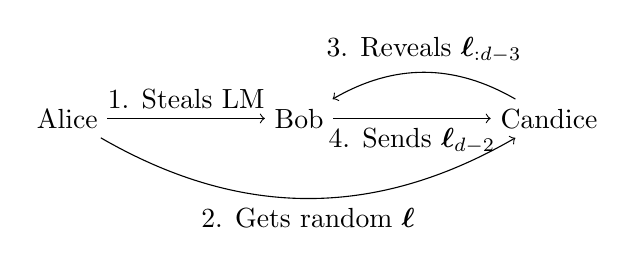
\begin{tikzpicture}[node distance=2cm]
    \node (A) {Alice};
    \node (B) [right=of A] {Bob};
    \draw[->] (A) -- node[above] {1. Steals LM} (B);
    \node (C) [right=of B] {Candice};
    \draw[->] (A) to[bend right] node [below] {2. Gets random \(\vell\)} (C);
    \draw[->] (C) to[bend right] node [above] {3. Reveals \(\vell_{:d-3}\)} (B);
    \draw[->] (B) to node [below] {4. Sends \(\vell_{d-2}\)} (C);
  \end{tikzpicture}
  \hfill
  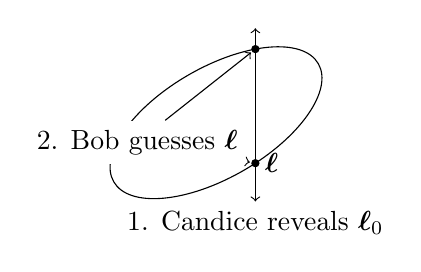
\begin{tikzpicture}[
      steplabel/.style={draw, fill=white},
      transformlabel/.style={fill=white, rounded corners, inner sep=1pt}
    ]
    \newcommand\yradius{0.7}
    \coordinate (input) at (0,0);
    \draw[name path=ellipse] (input) circle [x radius=1.5, y radius=\yradius, rotate=30];
    \draw[<->, name path=line] (0.5,1.2) -- (0.5,-1) node [below] {1. Candice reveals \(\vell_0\)};
    \fill [name intersections={of=ellipse and line}] 
    (intersection-1) circle (1.5pt) 
    (intersection-2) circle (1.5pt) node [right] {\(\vell\)};
    \node[fill=white] (B) at (-1, -0.25) {2. Bob guesses \(\vell\)};
    \draw[->, shorten >=2pt] (B) -- (intersection-1);
    \draw[->, shorten >=2pt] (B) -- (intersection-2);
  \end{tikzpicture}
\end{figure}



\bibliographystyle{chicago-annote}
\bibliography{refs}

\end{document}
